\documentclass{beamer}
\usetheme{Pittsburgh}

\usepackage[utf8]{inputenc}
\usepackage{default}
\usepackage[procnames]{listings}
\usepackage{graphicx}
%\usepackage[toc,page]{appendix}
\usepackage{caption}
\usepackage{hyperref}
\usepackage{color}
\usepackage{ulem}
%\usepackage{minted}


%Python
\definecolor{keywords}{RGB}{255,0,90}
\definecolor{comments}{RGB}{0,0,113}
\definecolor{red}{RGB}{160,0,0}
\definecolor{green}{RGB}{0,150,0}
\lstset{language=Python, 
    basicstyle=\ttfamily\scriptsize, 
    keywordstyle=\color{keywords},
    commentstyle=\color{comments},
    stringstyle=\color{red},
    identifierstyle=\color{green},
    procnamekeys={def,class},
    breaklines=true,
    columns=fullflexible,
    %Numbering and Tabs
    tabsize=4,
    showspaces=false,
    showstringspaces=false}

\begin{document}

\title{Python 2.7.6}
\subtitle{Object-Oriented Programming Concepts, Non-Primitive Data Types, and Generics}
\author{
  Mallick, Arka\\
  Naazare, Menaka \\
  Nair, Deebul\\
  Quignon, Christophe \\
} 
\institute{Hochschule Bonn Rhein Sieg}
\date{\today}

\begin{frame}
\titlepage
\end{frame}

%MENAKA
\begin{frame}[fragile]
\frametitle{classes, instances, objects}
\framesubtitle{}

\begin{itemize}
	\item Class is a blue print for a particular type of an object.
	\item An instance is a specific copy of the class that does contain all of the content. 
\item An object is an instance of a class.
\end{itemize}

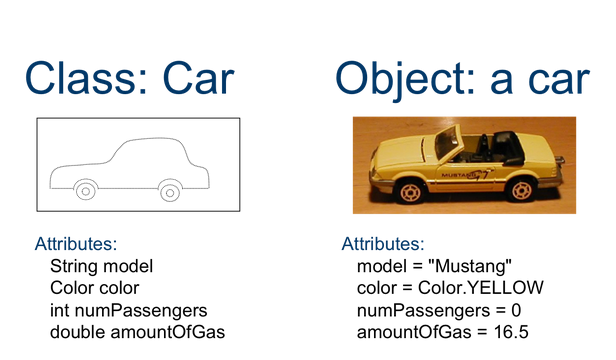
\includegraphics[width= 8cm]{1.png}
\end{frame}
%Menaka
\begin{frame}[fragile]

\frametitle{classes, instances, objects}
\begin{itemize}
\framesubtitle{}

\item What can you do with classes? 
		\begin{itemize}
		\item define your own classes 
\item inherit from your own or built-in classes 
\item instantiate the classes you've defined.
		\end{itemize}
	\item Defining a class
		\begin{itemize}
		\item Simplest way, reserved keyword class followed by a name(ofcourse with a semicolon at the end)
 		\end{itemize}
 	\item Inheriting from a class
 	\begin{itemize}
\item the ancestor of a class is simply listed in parentheses immediately after the class name 
\end{itemize}
\item Instantiating classes already defined
\begin{itemize}
\item Creating an instance of a class, creates an object of that class
\end{itemize}
\end{itemize}
\end{frame}

%MENAKA
\begin{frame}[fragile]
\begin{itemize}
\item Attribute is nothing but a variable which helps us to get from one object to another.
\item E.g of predefined attributes in python are dict, name, bases, doc, module.
\item Two types of attributes are :
\begin{itemize}
\item Class Attributes: An attribute defined in the class
\item Instance Attributes : An attribute defined in the instance.
\end{itemize}
\end{itemize}
\frametitle{Attributes}
\framesubtitle{}

\end{frame}

%CHRIS
\begin{frame}[fragile]
\frametitle{Types and \sout{Modifiers}}
No explicit typing, no hiding.\\
\huge \begin{quote}We are all consenting adults\end{quote}
\scriptsize \href{http://docs.python-guide.org/en/latest/writing/style/}{docs.python-guide.org/en/latest/writing/style}\\
\normalsize
\hbox{}
In Python all variables have a type.\\
The type is determined at runtime.\\
\hbox{}
\hbox{}
\hbox{}
\hfill Just in case...
\end{frame}

\begin{frame}[fragile]
\frametitle{Methods and Arguments }

\begin{verbatim}
def f( p, keyword='default', *positional, **optional):
  ...
\end{verbatim}

\begin{verbatim}classname.method(arguments)\end{verbatim}
\hbox{}
Arguments may be specified
\begin{itemize}
	\item positional
	\item keyworded
	\item default
	\item optional (as a dict)
	\item with arity 
\end{itemize}
\end{frame}



\begin{frame}[fragile]
\frametitle{Return, Assign and Polymorphism}%lists, return types, modifiers, variable arity methods, defaults
Return and assign works just like variable handling:
\begin{itemize}
	\item any types
	\item arbitrary many as tuple
	\item mangle
	\item polymorphism for free
\end{itemize}
\hbox{}
Convention and syntactic sugar:
\begin{itemize}
	\item pass
	\item \_ (be careful)
\end{itemize}

\end{frame}

\begin{frame}[fragile]
\frametitle{Inheritance and Overriding}
Classes can inherit from multiple other classes and thereby inherit their functions.

\begin{quote}
\begin{verbatim}
class DerivedClassName(BaseClassName):
\end{verbatim}\end{quote}
\hbox{}

magic methods overwrite these expressions/methods:
\begin{itemize}
	\item \_\_init\_\_
	\item \_\_lt\_\_
	\item \_\_iter\_\_
	\item \dots
\end{itemize}
$\rightarrow$ \href{http://www.rafekettler.com/magicmethods.html}{rafekettler.com/magicmethods}
\end{frame}

%DEBUL
\begin{frame}[fragile]
\frametitle{non-primitive data types}
\begin{itemize}
	\item Lists
	\item Tuples and Sequences
	\item Sets
	\item Dictionaries
	\item Looping Techniques
\end{itemize}
\framesubtitle{}

\end{frame}

%DEBUL
\begin{frame}[fragile]
\frametitle{Non-Primitive Data Types}
\framesubtitle{Lists}
\begin{itemize}
	\item list.append(x)
		\begin{itemize}
		\item Add an item to the end of the list;
		\end{itemize}
	\item list.extend(L)
		\begin{itemize}
		\item Extend the list by appending all the items in the given list; 		\end{itemize}

	\item list.insert(i, x)
		\begin{itemize}
		\item Insert an item at a given position. The first argument is the 				index of the element before which to insert
		\end{itemize}

	\item list.remove(x)
		\begin{itemize}
		\item Remove the first item from the list whose value is x. It is an 				error if there is no such item.
		\end{itemize}

	\item list.pop([i])
		\begin{itemize}
		\item 	Remove the item at the given position in the list, and 					return it. If no index is specified, a.pop() removes and 					returns the last item in the list. 
		\end{itemize}

\end{itemize}


\end{frame}

%DEBUL
\begin{frame}[fragile]
\frametitle{Non-Primitive Data Types}
\framesubtitle{Lists}
\begin{itemize}
	\item list.index(x)
		\begin{itemize}
		\item Return the index in the list of the first item whose value is x. It is an error if there is no such item.
		\end{itemize}

	\item list.count(x)
		\begin{itemize}
		\item Return the number of times x appears in the list.
		\end{itemize}

	\item list.sort()
		\begin{itemize}
		\item Sort the items of the list, in place.
		\end{itemize}
	
	\item list.reverse()
		\begin{itemize}
		\item Reverse the elements of the list, in place.
		\end{itemize}
\end{itemize}


\end{frame}

%DEBUL
\begin{frame}[fragile]
\frametitle{Non-Primitive Data Types}
\framesubtitle{Set}
A set object is an unordered collection of distinct hashable objects. Common uses include membership testing, removing duplicates from a sequence, and computing mathematical operations such as intersection, union, difference, and symmetric difference
\begin{itemize}
	\item add(elem)
		\begin{itemize}
		\item Add element elem to the set.
		\end{itemize}

	\item remove(elem)
		\begin{itemize}
		\item Remove element elem from the set. Raises KeyError if elem is not contained in the set.
		\end{itemize}

	\item discard(elem)
		\begin{itemize}
		\item Remove element elem from the set if it is present.
		\end{itemize}
	
	\item pop()
		\begin{itemize}
		\item Remove and return an arbitrary element from the set. Raises KeyError if the set is empty.
		\end{itemize}
		
	\item clear()
		\begin{itemize}
		\item Remove all elements from the set
		\end{itemize}
\end{itemize}


\end{frame}


%DEBUL
\begin{frame}[fragile]
\frametitle{Non-Primitive Data Types}
\framesubtitle{Dictionary}

\begin{itemize}
	\item Dictionaries are indexed by keys, which can be any immutable type
		\begin{itemize}
		\item Strings and numbers can always be keys. 
		\item Tuples can be used as keys if they contain only strings, numbers, or tuples
		\item If a tuple contains any mutable object either directly or indirectly, it cannot be used as a key
		\item You can’t use lists as keys, since lists can be modified in place using index assignments, slice assignments, or methods like append() and extend().
		\end{itemize}

	\item Dictionary is an unordered set of key: value pairs, with the requirement that the keys are unique (within one dictionary).
		

	\item The main operations on a dictionary are storing a value with some key and extracting the value given the key.
		
	
		
\end{itemize}


\end{frame}
%DEBUL
\begin{frame}[fragile]
\frametitle{Generic data types}
Python is a dynamically typed language, so it doesn't need generics. It can do something like this

\begin{verbatim}
	class BinaryTree:
    def __init__(self, left, right):
        self.left, self.right = left, right
\end{verbatim}
And it could be used like this:
\begin{verbatim}
	branch1 = BinaryTree(1,2)
	myitem = MyClass()
	branch2 = BinaryTree(myitem, None)
	tree = BinaryTree(branch1, branch2)
\end{verbatim}
\framesubtitle{}

\end{frame}

%\begin{frame}
% \frametitle{references}
% \begin{itemize}
%  \item Mark Lutz. 2003. Learning Python (2 ed.). O'Reilly \& Associates, Inc., Sebastopol, CA, USA.
%  \item \href{https://docs.python.org/2.7/}{docs.python.org/2.7/}
%  \item \href{http://interactivepython.org}{interactivepython.org}
% \end{itemize}
%\end{frame}
	

%COPY AND PASTE FROM HERE

%\begin{enumerate}
% \item 
%\end{enumerate}

%\hyperref{link}{text}

%\begin[Language=Python]{lstlisting}
%#PYTHON CODE HERE
%\end{lstlisting}

%\lstinputlisting[Language=Python]{ }

%\begin{figure}
% \center
% \includegraphics[width= cm]{img/ }
% \caption{}
%\end{figure}

%BIBLIOGRPAHY?
%\bibliographystyle{ieee}%amsalpha
%\bibliography{ }


\end{document}
